\chapter{CƠ SỞ LÝ THUYẾT}
\section{Khái niệm chung về mô hình mạng neural nhân tạo:}
Hệ thống mạng neural nhân tạo (Artificial Neural Network - ANN), hay gọi tắt là mạng neural, là một mô hình tính toán và xử lý thông tin được mô phỏng dựa trên cơ chế hoạt động hệ thống thần kinh của động vật. Cấu trúc của một mô hình mạng neural bao gồm nhiều nút neural được kết nối với nhau để xử lý thông tin thông qua việc truyền dẫn và tính toán các giá trị mới tại các neural đó. Có cơ chế tương tự não người, mô hình mạng neural cũng có thể học hỏi thông qua huấn luyện các kiến thức chưa biết và ứng dụng nó để dự đoán các dữ liệu chưa biết đến.

\begin{figure}[htbp]
    \centering
    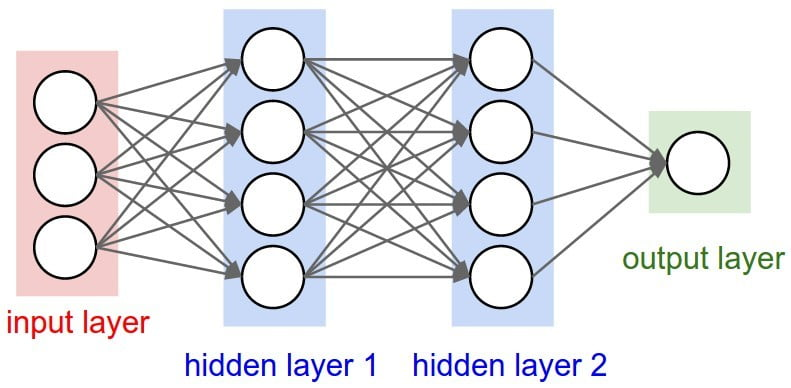
\includegraphics[width=12cm]{Images/ANN.jpg}
    \caption[Kiến trúc tổng quan của mô hình mạng thần kinh]
    {Kiến trúc tổng quan của mô hình mạng thần kinh - Stanford CS231n}
\end{figure}
\newpage
Trong một hệ thống mạng neural, các neural được phân làm 3 lớp chính khác nhau, bao gồm: Input Layer, Hidden Layer và Output Layer. Input Layer là lớp tiếp nhận các dữ liệu đầu vào và tiền xử lý dữ liệu. Lớp Hidden Layer thực hiện các bước rút trích, phân tích và tính toán các luồng dữ liệu nhận từ Input Layer, và có thể có một hoặc nhiều lớp khác nhau trong một hệ thống mạng neural. Còn lớp Ouput Layer có nhiệm vụ trả dữ liệu đầu ra của hệ thống, ví dụ như kết quả phân loại của một mô hình phân loại dữ liệu. Thông thường quá trình suy luận từ Input Layer cho đến tới Output Layer của mô hình mạng neural là quá trình lan truyền tiến (feedforward), tức là đầu vào các neural tại một lớp đều lấy từ kết quả các neural lớp trước đó mà không có quá trình suy luận ngược lại.

Ngoài ra, những kết nối giữa các neural còn được liên kết với một trọng số để thể hiện mức độ quan trọng của dữ liệu đầu vào trong quá trình xử lý thông tin cũng như quá trình chuyển đổi dữ liệu từ lớp này đến lớp khác. Thực chất, quá trình học của mạng neural chính là quá trình cân chỉnh trọng số liên kết giữa các kết nối cũng như từ dữ liệu đầu vào để đưa ra kết quả mong muốn.

\begin{figure}[htbp]
    \centering
    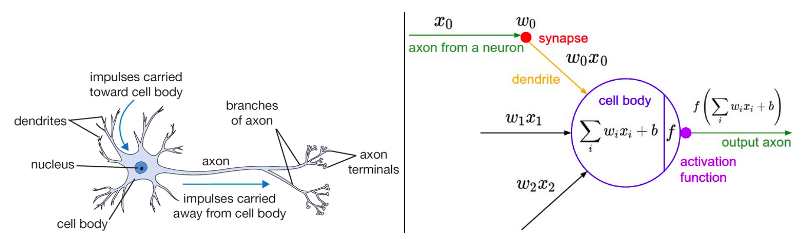
\includegraphics[width=13cm]{Images/neural.png}
    \caption[Cấu tạo của neural trong sinh học và trong mô hình ANN]
    {Cấu tạo của neural trong sinh học và trong mô hình ANN - Stanford CS231n}
\end{figure}

Cấu trúc của một neural bao gồm một hàm tổng (Summation Function) có vai trò tính toán các dữ liệu đầu vào cùng với trọng số có sẵn để đưa ra dữ liệu kết quả của neural đó. Kết quả này sẽ được đưa qua môt hàm kích hoạt (Activation Function) để quyết định xem neural đó có được phép hoạt động và cập nhập dữ liệu mới trên mô hình mạng hay không. Hàm kích hoạt giúp mô hình mạng neural có thể học hỏi được các mối quan hệ của dữ liệu hay thực hiện các tác vụ phức tạp khác, mà đa phần không phải là tuyến tính. Chính vì vậy, các hàm kích hoạt đều là hàm phi tuyến. Tùy thuộc vào hàm kích hoạt khác nhau sẽ có các công thức hàm khác nhau, ví dụ như hàm kích hoạt Sigmoid có công thức như sau:

\begin{equation*}
f_{S}(x) = \frac{1}{1 + e^{x}}\\
\end{equation*}
